\documentclass{article}
\usepackage[utf8]{inputenc}
\usepackage[margin= 1in]{geometry}
\usepackage[utf8]{inputenc}
\usepackage[none]{hyphenat}
\usepackage{parskip}
\usepackage{multicol}

\usepackage{listings}  
\usepackage[numbered,framed]{matlab-prettifier}
\usepackage[T1]{fontenc}
% standard packages
\usepackage{subcaption}
\usepackage{enumerate}
\usepackage{nccmath}
\usepackage{svg}
\usepackage{mathtools}
\usepackage{scalerel,stackengine}
\stackMath
\newcommand\reallywidehat[1]{%
\savestack{\tmpbox}{\stretchto{%
  \scaleto{%
    \scalerel*[\widthof{\ensuremath{#1}}]{\kern-.6pt\bigwedge\kern-.6pt}%
    {\rule[-\textheight/2]{1ex}{\textheight}}%WIDTH-LIMITED BIG WEDGE
  }{\textheight}% 
}{0.5ex}}
\stackon[1pt]{#1}{\tmpbox}%
}
\parskip 1ex
\usepackage{float}
\usepackage{scrextend}
\usepackage{fancyhdr}
\usepackage{fancyvrb}
%\usepackage{bickham}
% \usepackage{BOONDOX-cal[o]}
%\usepackage{boondox-calo}
% \usepackage{dutchcal}
\usepackage{minted}
\usepackage{hyperref}
% math packages
\usepackage{centernot}
\usepackage{amsthm, amssymb, amsmath,verbatim}
\usepackage{mathtools}
% coding and colors
\usepackage{xifthen}
\usepackage{xcolor}
\usemintedstyle{borland}
\usepackage{ifthen}

% color box
\usepackage[most,listings]{tcolorbox}
\usepackage{lmodern}
% graphs and pictures
\usepackage{mathrsfs}
\usetikzlibrary{math}
\usetikzlibrary{backgrounds}
\usetikzlibrary{patterns,calc}
\usepackage{subcaption}
\usepackage[demo]{graphicx}
\usepackage{csvsimple,booktabs}
\usepackage{filecontents}
\theoremstyle{definition}
\newtheorem{definition}{Definition}[section]
\newtheorem{theorem}{Theorem}[section]
\newtheorem{assmp}{Assumption}[section]
\usepackage{geometry}
\geometry{
	%margin = 14.11mm, tmargin = 0.4 in
	margin = 15mm, bmargin = 0.in, tmargin = 0.4in
}

%\usepackage{bbm}
\usepackage{authblk}

\usepackage{mathtools}

\newcommand{\R}{\mathcal{R}}
\newcommand{\SA}{\mathcal{S}}
\newcommand{\E}{\mathcal{E}}
\newcommand{\F}{\mathcal{F}}
\newcommand{\U}{\mathcal{U}}
\usepackage[ruled,vlined]{algorithm2e}
\usepackage{algorithm,algpseudocode}
\def\course{Course \#: Course Title}      %Course
\def\thetitle{Report Title}               % Report Title
\def\Headauthor{last name et al.}         % Header Authors of work
\def\date{\today}                         % Date
\usepackage{array}
\newcommand{\PreserveBackslash}[1]{\let\temp=\\#1\let\\=\temp}
\newcolumntype{C}[1]{>{\PreserveBackslash\centering}p{#1}}
\newcolumntype{R}[1]{>{\PreserveBackslash\raggedleft}p{#1}}
\newcolumntype{L}[1]{>{\PreserveBackslash\raggedright}p{#1}}

\begin{document}

\begin{center}
    \vspace*{1.5cm}
    % University Logo
    
\includegraphics[scale = 0.5]{iitb-logo.png}\\[1.75cm]
    % University Name
    \textsc{\color[RGB]{0, 51, 102}\LARGE{Indian Institute of Technology Bombay}}\\[1cm]
    {\Large{CS 769 Course Project }}\\[.5cm]
   {\Large{Combinatorial Optimization using Reinforcement Learning}}\\[.5cm]
    \textsc{\date}\\[2cm]
    \Large{
    \begin{tabular}{L{5cm} R{4cm}}
        \textit{Author} &  \textit{Roll Number}\\
        % \hline
        % author names and PID
        Tejas Pagare & 190070067\\
        Kaustubh Ponkshe & 190100064
    \end{tabular}
    }\\
    \vspace{1cm}
    \textit{under the guidance of}
    \\\vspace{1cm}
    Prof. Ganesh Ramakrishnan\\
    \vspace{0.2cm}
    % \textit{Electrical Engineering, IIT Bombay}\\[.5cm]
    
\end{center}
\thispagestyle{empty}
\pagebreak

\newgeometry{
	a4paper,margin = 20mm,top=25mm,bottom=25mm,bindingoffset=6mm
}
\clearpage
\pagestyle{fancy}
\tableofcontents
\clearpage
\section{Introduction}
In this project, we explore the topic of combinatorial optimization. Combinatorial optimization is an optimization problem with discrete objects and the objective of the algorithm is to minimize or maximize a cost function. The problem is to find an optimal solution from a feasible set of discrete finite solutions. Some examples of combinatorial optimization include Travelling salesman-problem, minimum graph cut, set cover problem, etc. The applications of these problems are broad, ranging from logistics, kidney donation chaining to computer vision and water distribution. However the major problem in solving these algorithms is that they are NP hard problems. However, we can do better in the following ways :
\begin{enumerate}
    \item Polynomial time exact solvers for some subsets of problems
    \item Polynomial time algorithms which approximately solve the optimization upto some degree of performance worse than the optimal solution
    \item Heuristic based algorithms which train using trial and error and learn heuristics
    
\end{enumerate}
We will be focusing on the heuristic based algorithms and will look at a few examples of algorithms applied specifically to the travelling salesman problem. The development of excellent heuristics or approximation algorithms for NP-hard combinatorial optimization problems necessitates a great deal of specialised expertise and trial-and-error. Our aim is to automate these algorithms. \\

In many real-world applications, the same optimization issue is addressed over and over again on a regular basis, with the same problem structure but different data each time. This opens the door to developing heuristic algorithms that take use of the structure of such reoccurring situations.Heuristics are frequently quick, effective algorithms with no theoretical guarantees, and they may also need extensive problem-specific study and trial-and-error on the side of method inventors. The three described methods, however, rarely take use of a common feature of real-world optimization problems: instances of the same type of issue are addressed on a frequent basis, with the same combinatorial structure but mostly different input. In many cases, the values of the objective function's coefficients or restrictions may be regarded of as being sampled from the same underlying distribution.\\

In this work, we will compare various greedy and heuristic based strategies to solve the Travelling salesman problem. In particular, we will explore the methods involved and advantages of using deep learning to learn the huersitics and aid in particular algorithms. 

\begin{figure}[H]
    \centering
    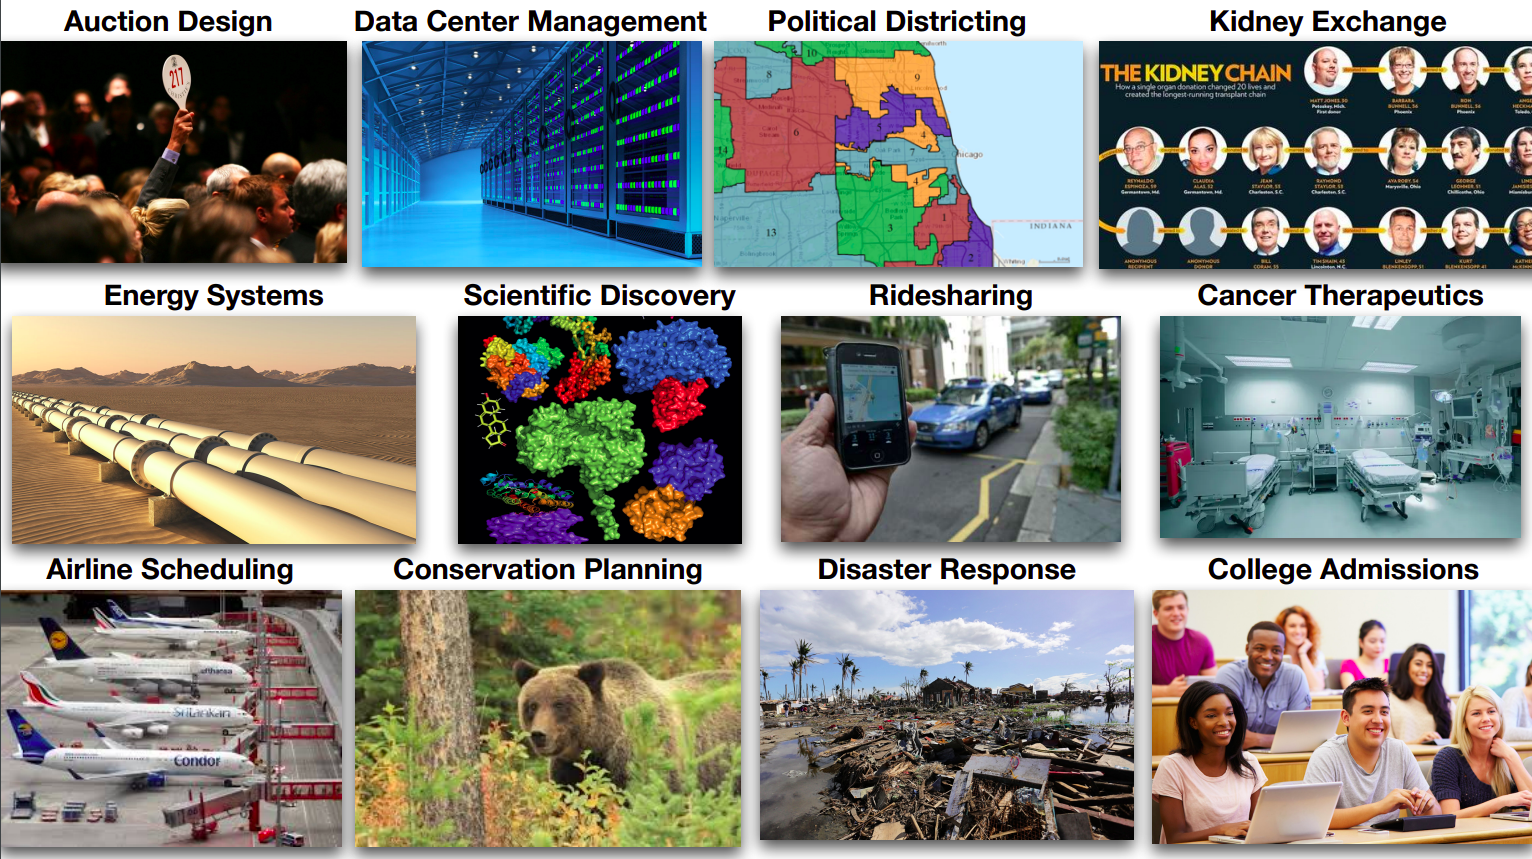
\includegraphics[width=0.8\textwidth]{images/Applications.png}
    \caption{Applications of Combinatorial Optimization in a nutshell \cite{tutorial}}
    \label{fig:my_label}
\end{figure}
\section{Background}
Suppose you are scientist and you are attending a conference. You want to visit all the posters and return back to where you started from by travelling the minimum distance. However, this we note is exactly the Travelling Salesman Problem, which is known to be NP-hard. To formalize this,\\


\textbf{Travelling Salesman Problem}:\emph{"Given a set of points in 2-dimensional space, find a tour
of minimum total weight, where the corresponding graph $G$ has the points as nodes and is fully
connected with edge weights corresponding to distances between points; a tour is a cycle that visits each node of the graph exactly once"}\\

Consider a graph $G= (V,E) $ where $V = (v_1, v_2, ...v_n)$ is a set of n vertices and there is a cost function $c_{ij}$ associated with each edge $e_{ij} \in E$. Now consider variables $x_{ij}$ such that .
$$ 
x_{ij} =
\begin{cases}
    1 \text{  if there is a path from i to j}\\    
 0  \text{  otheriwse}
\end{cases} $$
Then our optimization problem can be given as 
$$ \text{min } \sum_{i=1}^n  \sum_{i \neq j,j=1}^n x_{ij}c_{ij}$$
with the constraint that 
$$  \sum_{i=1,i \neq j}^n x_{ij}=1, \text{ for every $j$ and }  \sum_{i \neq j,j=1}^n x_{ij}=1  \text{ for every $i$} $$
\\
The problem can be represented as a graph, with each node representing the coordinate of the vertex. The graph is assumed to be fully connected. We will first go over the greedy algorithms used and their performance. Then we will list out some heuristic based algorithms where the heuristic shave been preset. Finally we will look at examples of learning heuristics for these algorithms. \\
Typically, many combinatorial problems can be represented by graphs and this makes it possible to share heuristics between related problems. In fact we will show that even the hyperparameters can be transferred across tasks. Took take few examples consider:\\


\textbf{Minimum Vertex Cover (MVC)}:\emph{" Given a graph $G$, find a subset of nodes $S \subseteq V$ such that every edge is covered, i.e. $(u, v) \in E \iff u \in S$ or $v \in S$, and |S| is minimized"}\\

\textbf{Maximum Cut (MAXCUT)}:\emph{"Given a graph G, find a subset of nodes $S\subseteq V$ such that the weight
of the cut-set $\sum\limits_{(u,v) \in C} w(u, v)$ is maximized, where cut-set $ C \subseteq E$  is the set of edges with one
end in S and the other end in V \textbackslash S."}\\


\section{Greedy and Heuristic based algorithms}
To start of for the task of solving the travelling salesman problem, we chose nearest neighbour algorithm (greedy algorithm) to see the results. Greedy algorithms are a class of algorithms which look for best in the short run, whether or not it is best in the long run.Greedy algorithms optimize locally, but not necessarily globally. They don't necessarily converge to optimal solution ( although in some cases, we can give error bounds) but are usually very fast and simple. We will define the nearest neighbour algorithm as follows\\

\emph{"The Nearest-Neighbor Algorithm begins at any vertex and follows the
edge of least weight from that vertex. At every subsequent vertex, it
follows the edge of least weight that leads to a city not yet visited, until
it returns to the starting point."}

The average cost of such greedy algorithms has been found to be only a constant proportional worse than the optimal solution, however the worst case solutions can be abitrarily bad. 

% \begin{algorithm}[H]
%  \KwData{$x_1\in F,\text{ step size } \alpha\ ,\beta_1, \beta_2 $}

%  \For{t=1 to T}{
%   g_t = \triangledown f_t(x_{t})\\
%  m_t = \beta_1 m_{t-1} + (1-\beta_1) g_t\\
%   v_t = \beta_2 v_{t-1} + (1-\beta_2) g_t^2\\
%   \hat{m}_t = m_t/(1-\beta_1^t)\\
%   \hat{v}_t = v_t/(1-\beta_2^t)\\
%   x_{t} = x_{t-1} - \alpha \hat{m}_t / (\sqrt{\hat{v}_t} + \epsilon) \\
%  }
%  \EndFor
%  \caption{ADAM}

%\end{algorithm}
Besides this, we will also go over two heuristic based  (but not learning based) algorithms, namely the nearest insertion and the farthest insertion algorithms. 

\begin{algorithm}[H]

\SetAlgoLined
\textbf{Select} $v_1\in V,\text{Intitialize subgraph}\ S= \phi$\\
\text{Find vertex} $v_j = \underset{v_j}{\text{argmin}}\ c_{1j}$ \Comment{vertex closest to $v_1$} \\
$ S= \{v_1,v_j,v_1\}$\Comment{partial solution} \\
\For{t=1 to n-2}{
  Find vertex $v_k = \underset{v_i \in S}{\text{argmin}}\ c_{ik}$ \Comment{vertex closest to all nodes in $S$}\\
  \text{Find arc} $(i,j) = \underset{v_i,v_j \in S}{\text{argmin}}\ c_{ik} + c_{kj}- c_{ij}$\\
  \text{Update}  $S= \{v_1,\ldots,v_j,v_k,v_i,\ldots,v_1\}$ \Comment{insert $v_k$ between $v_i$ and $v_j$}
 }
 \EndFor
 \caption{Nearest Insertion Algorithm}

\end{algorithm}
The farthest insertion can be given by chosing the farthest vertex rather than the nearest one.

\subsection{Experimental Results}
Following are experimental results for the Traveling Salesman Problem
\begin{center}
\begin{tabular}{|c|c|c|c|}
\hline
    Nodes & Nearest Neighbour &  Nearest Insertion & Farthest Insertion\\\hline
    20 & 5.106 & 5.248 & 5.246\\\hline
    50 & 7.293  & 7.378 & 8.076\\\hline
\end{tabular}
\end{center}
\begin{figure}[!htb]
\minipage{0.32\textwidth}
  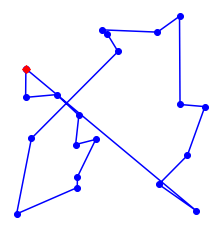
\includegraphics[width=0.7\linewidth]{images/nn20.png}
  \caption*{Nearest Neighbour}\label{fig:awesome_image1}
\endminipage\hfill
\minipage{0.32\textwidth}
  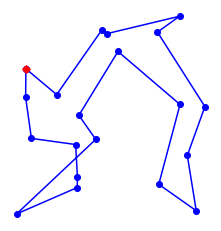
\includegraphics[width=0.7\linewidth]{images/ni20.png}
  \caption*{Nearest Insertion}\label{fig:awesome_image2}
\endminipage\hfill
\minipage{0.32\textwidth}%
  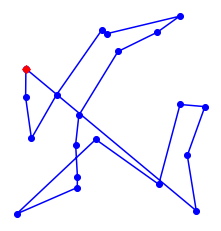
\includegraphics[width=0.7\linewidth]{images/fi20.png}
  \caption*{Farthest Insertion}\label{fig:awesome_image3}
\endminipage
\caption{20 nodes\\
red vertex indicates the starting and hence ending point}
\end{figure}
\section{Learning Methods}
As can be seen from the above algorithms it is quite cumbersome to come with a good heuristic to solve CO problems and in most cases it is problem dependent. Now, we will move to some techniques which aims to learn the heuristic for CO problems. This is where we encapsulate Reinforcement Learning where a particular CO problem can be adopted as an environment which provides rewards/cost for each action taken by an agent and the agent has to explore and exploit the information gathered from the environment interaction in order to optimize the objective.
\subsection{Reinforcement Learning}
First of all, to use Reinforcement Learning, a CO problem has to modeled as an sequential decision problem in particular as a Markov Decision Process exploiting the Markov Property which holds in most scenarios

\begin{definition}[Controlled Markov Property]
\[\text{Pr}\{X_n=j|X_m,U_m,m< n\} = \text{Pr}\{X_n=j|X_{n-1}=i,U_{n-1}=a\}\]
which says that state $X_n$ is independent of past states and actions given the last state $X_{n-1}$ and action $U_{n-1}$.
\end{definition}
\begin{definition}[Markov Decision Process]
A MDP consists of 
\begin{itemize}
    \item A set of states $\mathcal{S}$, set of actions $\mathcal{A}$ for moving from a state to another. $\mathcal{S}$ and $\mathcal{A}$ can be both finite or infinite.
    \item Transition Probabilities $P$ which is defined the probability distribution over next states given the current state and current action where $P_{ij}(a) = \text{Pr}\{X_{n+1}=j|X_{n}=i,U_n=a\}$.
    \item A reward function which is defined as $\mathcal{R}: \mathcal{S}\times\mathcal{A}\rightarrow\mathbb{R}$, where $\mathcal{R}_s^a$ or $r(s,a)$ is the expected reward of taking action $a$ in state $s$.
\end{itemize} 

Therefore a MDP is simply given as a pair $(\mathcal{S},\mathcal{A},\mathcal{R})$.\\
\end{definition}
A policy $\pi:\mathcal{S}\rightarrow\mathcal{A}$ is a distribution over actions given states $\pi(a|s) = \text{Pr}\{U_n=a|X_n=s\}$. \\For stationary policy we have $U_n\sim \text{Pr}(\cdot|X_n=s)$ $\forall t>0$.\\
Any policy induces a Markov chain whose transition probability or stochastic matrix is denoted as $P(\pi) \in [0,1]^{|\mathcal{S}|\times|\mathcal{S}|}$  where each entry $P_{ij}(\pi) = \sum_{a\in\mathcal{A}}\pi(a|s)p(j|i,a)$. This Markov chain is denoted as $(\mathcal{S},\mathcal{P}(\pi))$.\\

\begin{figure}[H]
    \centering
    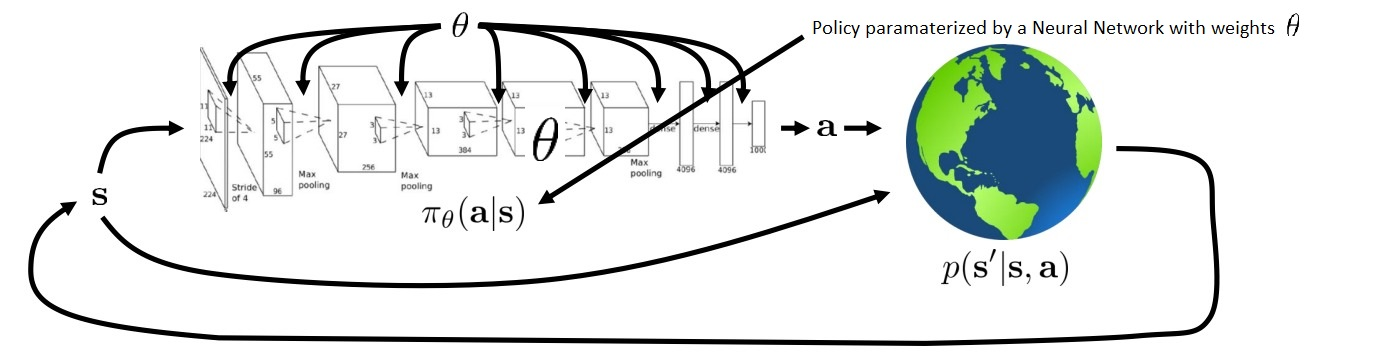
\includegraphics[width=15cm]{images/rl.jpeg}
    \caption{Agent-Environment Interaction \cite{sergey}}
    \label{fig:my_label}
\end{figure}

Objective of Reinforcement Learning is to maximize (minimize) the expected long run reward (cost) formally defined as finding
\[\theta^\star = \underset{\theta}{\text{argmax}}\mathbb{E}_{\tau\sim p_\theta(\tau)}\Big[\sum_t r(s_t,a_t)\Big]\]
where 
\[p_\theta(s_1,a_t,\ldots,s_T,a_T)=p(s_1)\prod_{t=1}^T\pi_\theta(a_t|s_t)p(s_{t+1}|s_t,a_t)\]
where $T$ can be infinite.\\

Now, we will explore a particular Reinforcement Learning algorithm called REINFORCE \cite{Sutton1998} which belongs to the family of Policy Gradient algorithms
\subsubsection{REINFORCE Algorithm}
We will first state a generalization of policy gradient theorem with a baseline (reduces variance)
\begin{theorem}[Policy Gradient Theorem]
\begin{equation}
\label{eq:pg}
    \nabla J(\theta) \propto \sum_s \mu(s) \sum_a\Big(Q_\pi(s,a)-b(s)\Big)\nabla \pi_\theta(a|s)=\mathbb{E}_\pi\Big[\sum_a\Big(Q_\pi(s,a)-b(s)\Big)\nabla \pi_\theta(a|s)\Big]
\end{equation}
where $J(\theta)=\mathbb{E}_{\tau\sim p_\theta(\tau)}\Big[\sum_t r(s_t,a_t)\Big]$ and \[Q_\pi(s,a)=\mathbb{E}_\pi[G_t|S_t=s,A_t=a]=\mathbb{E}_\pi\Big[\sum_{k=0}^\infty\gamma^k R_{t+k+1}|S_t=s,A_t=a\Big]\]
is the Q-value function for policy $\pi$ and $\mu(s)$ is a state distribution satisfying $\mu(s)\geq0\ \forall\ s$ and $\sum_s\mu(s)=1$.
\end{theorem}

In Eq.\eqref{eq:pg}, the baseline $b(s)$ can be in general any random variable depending on $s$ and the most common and natural choice is to use an estimate of the state-value function i.e. $\hat{V}(s)$ generally a parameterized function $\hat{V}(s,\textbf{w})$ with weight vector $\textbf{w}\in \mathbb{R}^d$.\\

The policy-gradient methods seek to maximize the perform ace using the stochastic gradient \emph{ascent} in $J$ as follows:
\[\theta_{t+1}=\theta_t+\alpha\reallywidehat{\nabla J(\theta_t)}\]
where $\reallywidehat{\nabla J(\theta_t)}$ is the stochastic estimate of the actual gradient of $J$ w.r.t  $\theta$\\

REINFORCE is a policy gradient method which is based Monte-Carlo estimates to update the policy parameters $\theta$, the update is as follows
\[\theta_{t+1}=\theta_t+\alpha \Big(G_t-b(S_t)\Big)\dfrac{\nabla \pi_\theta(A_t|S_t)}{\pi_\theta(A_t|S_t)}\]
\begin{algorithm}[H]
\SetAlgoLined
\caption{REINFORCE with Baseline (episodic), for estimating $\pi_\theta\approx\pi_*$}
\textbf{Input}: a differentiable policy parameterization $\pi_\theta(a|s)$, a differentiable state-value function parameterization $\hat{V}(s,w)$\\
Algorithm parameters: step sizes $\alpha_1 > 0, \alpha_2 > 0$\\
Initialize policy parameter $\theta\in\mathbb{R}^{d'}$ and state-value parameters $w\in\mathbb{R}^d$\\
\For{\text{each episode}}{
Generate an episode $S_0, A_0, R_1,\ldots,S_{T-1},A_{T-1},R_T,$ following $\pi_\theta(\cdot|\cdot)$\\
\For{\text{step} t=0,1,\ldots,T-1}{
$G\gets \sum_{k=t+1}^T\gamma^{k-t-1}R_k$\\
$\delta\gets G-\hat{V}(s,w)$\\
$w\gets w+\alpha_1\delta\nabla\hat{V}(S_t,w)$\\
$\theta\gets\theta+\alpha_2\gamma^t\delta\nabla\text{ln}\pi_\theta(A_t|S_t)$
}}
\end{algorithm}

\subsection{Attention Based REINFORCE Algorithm}
Now, we will explore the paper \cite{attention} which uses an encoder-decoder based architecture for the policy and applies REINFORCE for optimization.\\

Consider for the n-node graph problem instance $s$, the solution tour $\pi = (\pi_1,\ldots,\pi_n)$ as the permutation of nodes, $\pi_t\in\{1,\ldots,n\}$. The aim is to find a stochastic policy factorized using $p_\theta(\pi|s)=\prod_{t=1}^n p_\theta(\pi_t|s,\pi_{1:t-1})$.\\

The encoder produces the embedding for each node and the decoder produces the sequence $\pi$ of input nodes one at a time using the encoder node embeddings.
\subsubsection{Attention Model}
Here, we consider the an encoder-decoder architecture similar to Transformer \cite{https://doi.org/10.48550/arxiv.1706.03762}.\\

Encoder:
\begin{figure}[H]
    \centering
    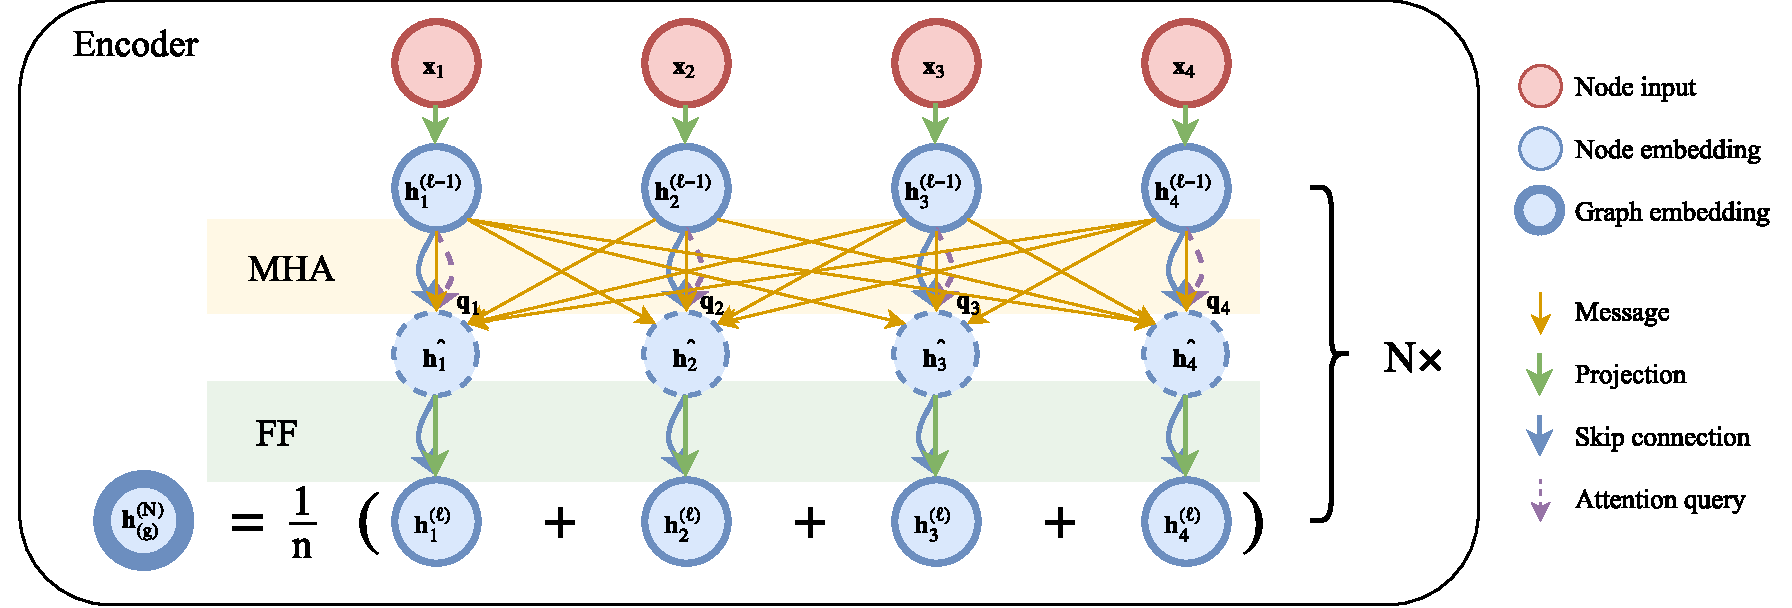
\includegraphics[width=8cm]{images/Encoder.pdf}
    \caption{Attention based encoder}
    \label{fig:my_label}
\end{figure}
Here for encoder we have\\
$x_i$ is $d_x$ dimensional input feature for node $i$ e.g. x,y coordinates for TSP.\\
$ \mathbf{h}_i^{(0)}$ is learned $d_h$ dimensional node embedding with parameters $W^x$ and $b^x$ as $ \mathbf{h}_i^{(0)}=W^xx_i+b^x$\\
Output is node embedding for each node $i$, $ \mathbf{h}_i^{(N)}$ and graph embedding $\bar{\mathbf{h}} ^{(N)}=\dfrac{1}{n}\sum_{i=1}^n  \mathbf{h}_i^{(N)}$\\
$ \mathbf{h}_i^{(l)}$ is the node embedding produced by the layer $l\in\{1,\ldots,N\}$

Each attention layer contains a Multi-Head Attention (MHA) and fully connected feed-forward (FF) layer same as the Transformer architecture and  skip-connection and batch normalization (BN):
\begin{align}
	 \hat{\mathbf{h}}_i & =\text{BN}^{\ell}\left( \mathbf{h}_i^{(\ell-1)} + \text{MHA}_i^{\ell}\left( \mathbf{h}_1^{(\ell-1)}, \ldots, \mathbf{h}_n^{(\ell-1)}\right)\right) \label{eq:attn_sublayer1} \\
    \mathbf{h}_i^{(\ell)} & =\text{BN}^{\ell}\left(\hat{\mathbf{h}}_i + \text{FF}^{\ell}(\hat{\mathbf{h}}_i)\right). \label{eq:attn_sublayer2}
\end{align}





Decoder:\\
Decoder outputs $\pi_t$ sequentially based on embeddings from the network and $\pi_{t'}$ for $t'<t$.\\

The graph is augmented with a special context node (c) which essentially tries to represent the decoding context. The context embedding is given as 
\begin{equation}
	\mathbf{h}_{(c)}^{(N)} = \begin{cases}
		\left[\bar{\mathbf{h}}^{(N)} , \mathbf{h}^{(N)}_{\pi_{t-1}} , \mathbf{h}^{(N)}_{\pi_1}\right] & t > 1 \\
        \left[\bar{\mathbf{h}}^{(N)} , \mathbf{v}^\text{l} , \mathbf{v}^\text{f}\right] & t = 1.
\end{cases} \\
\end{equation}
where $[\cdot,\cdot,\cdot]$ is the horizontal concatenation operator and $\mathbf{v}^\text{l} , \mathbf{v}^\text{f}$ are learned.\\

Now finally we perform two attention steps, first one uses Multi-Head Attention between context node and other nodes and later one is a single head attention to calculate the log-probabilities of the tour sequence.\\\

To compute the context node encoding $\mathbf{h}_{(c)}^{(N+1)}$ the keys and values are computed for each node using the node embeddings $\mathbf{h}_i^{(N)}$, and a single query $\mathbf{q}_{(c)}$ (per head) is computed:
\begin{equation}
\label{eq:dec_qkv}
	\mathbf{q}_{(c)} = W^Q \mathbf{h}_{(c)} \quad \mathbf{k}_i = W^K \mathbf{h}_i, \quad \mathbf{v}_i = W^V \mathbf{h}_i.
\end{equation}

To calculate the log-probabilities we first compute compatibilities $u_{(c)j}$, after clipping the result (before masking!) within $[-C, C]$ (C = 10) using $\tanh$:
\begin{equation}
\label{eq:dec_logits}
	u_{(c)j} = \begin{cases}
		C \cdot \tanh \left(\frac{\mathbf{q}_{(c)}^T \mathbf{k}_j}{\sqrt{d_{\text{k}}}}\right) & \text{if } j \neq \pi_{t'} \quad \forall t' < t \\
        -\infty & \text{otherwise.}
    \end{cases}
\end{equation}
We interpret these compatibilities as unnormalized log-probabilities (logits) and compute the final output probability vector $\mathbf{p}$ using a softmax:
\begin{equation}
	\label{dec:probabilities}
    p_i = p_{\bm{\theta}}(\pi_t = i|s, \bm{\pi}_{1:t-1}) = \frac{e^{u_{(c)i}}}{\sum_{j}{e^{u_{(c)j}}}}.
\end{equation}

\begin{figure}[H]
    \centering
    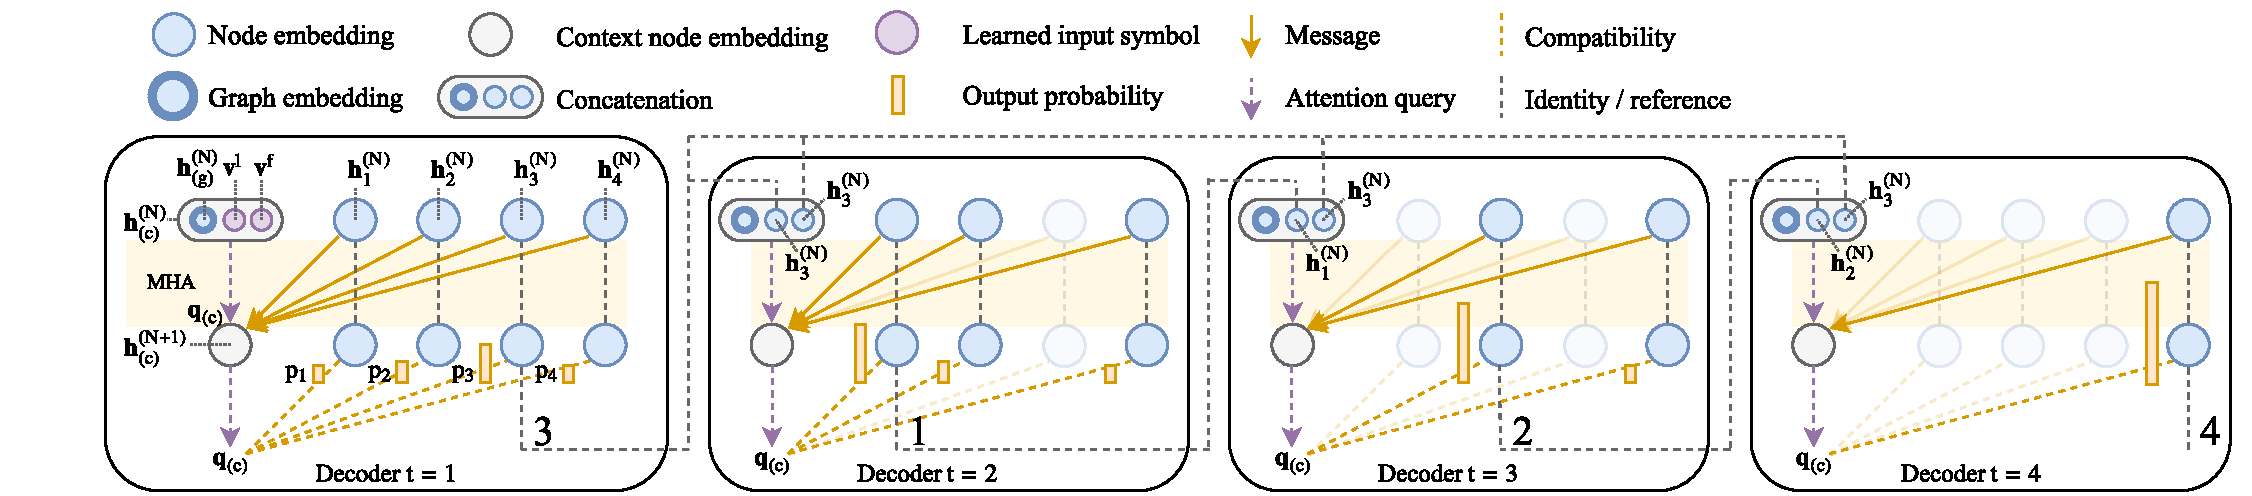
\includegraphics[width=15cm]{images/Decoder.pdf}
    \caption{Decoder with output tour as $\pi=$(3,1,2,4)}
    \label{fig:my_label}
\end{figure}

\subsubsection{REINFORCE}
For a given problem instance $s$, the encoder-decoder architecture outputs $\p_\theta(\pi|s)$ from which we sample a tour $\pi$ and define the loss as 
we sample a policy $\pi$ (permutation of nodes) to computed the loss defined as\\
\[\mathcal{L}(\theta|s)=\mathbb{E}_{p_\theta(\pi|s)}[L(\pi)]\]
We optimize $\mathcal{L}$ using gradient-ascent most commonly known as  REINFORCE where we have the gradient of the loss as
\[\nabla\mathcal{L}(\theta|s)=\mathbb{E}_{p_\theta(\pi|s)}[(L(\pi)-b(s))\nabla \text{log}p_\theta(\pi|s)]\]

A good baseline $b(s)$ reduces the gradient variance!\\
We use 2 baselines for the experimentation:
\begin{enumerate}
    \item greedy rollout baseline: defined as the cost of a solution of a deterministic greedy rollout policy by the best model so far
    \item critic: a function $\hat{V}(s,w)$ of state $s$, parameterized by $w$, which is learned using gradient ascent iteration similar to original REINFORCE iteration
\end{enumerate}
Intuition behind greedy rollout baseline: The policy gradient in REINFORCE has the term $L(\pi)-b(s)$ which is negative if the sampled solution $\pi$ is better that the greedy sampled baseline causing actions to be reinforced (hence the name) and vice versa. This indicated the improvement of the model from its \emph{greedy self}!
\\

The motivation behind choosing a baseline that it should estimate the difficulty of the problem instance $s$. \\
Based on the observation that the difficulty of a problem instance depends on the performance of an algorithm used for training motivates that the baseline should be defined by the model during training. \\
To eliminate the variance, the baseline is chosen greedily to the action with maximum probability. \\

Now, it is important to note that during the training process, model keeps changing and hence the baseline and hence it order to stabilize the basline it is kept frozen for fixed number of steps every epoch.\\
    The parameters associated with baseline policy $\bm{\theta}^{\text{BL}}$ is changed to policy parameters $\theta$ at the end of every epoch if current training policy is better compared to the baseline policy according to a paired t-test with significance $\alpha$.\\
    
The REINFORCE algorithm is fully described using the following pseudo-code
\begin{algorithm}[H]
\SetAlgoLined
  \caption{REINFORCE with Rollout Baseline} \label{alg:reinforce_rollout}
  \textbf{Input:}number of epochs $E$, steps per epoch $T$, batch size $B$, significance $\alpha$\\
    Init $\bm{\theta},\ \bm{\theta}^{\text{BL}} \gets \bm{\theta}$\\
      \For{$\text{epoch} = 1, \ldots, E$}{
        \For{$\text{step} = 1, \ldots, T$}{
        	 $s_i \gets \text{RandomInstance()} \enspace \forall i \in \{1, \ldots, B\}$\\
             $\bm{\pi}_i \gets \text{SampleRollout}(s_i, p_{\bm{\theta}}) \enspace \forall i \in \{1, \ldots, B\}$\\ $\bm{\pi}_i^{\text{BL}} \gets \text{GreedyRollout}(s_i, p_{\bm{\theta}^{\text{BL}}}) \enspace \forall i \in \{1, \ldots, B\}$\\ $\nabla\mathcal{L} \gets \sum_{i=1}^{B} \left(L(\bm{\pi}_i) - L(\bm{\pi}_i^{\text{BL}})\right) \nabla_{\bm{\theta}} \log p_{\bm{\theta}}(\bm{\pi}_i)$\\
             $\bm{\theta} \gets \text{Adam}(\bm{\theta}, \nabla\mathcal{L})$}

      \If{\text{OneSidedPairedT-Test}(p_{\bm{\theta}}, p_{\bm{\theta}^{\text{BL}}}) < \alpha}{
		 $\bm{\theta}^{\text{BL}} \gets \bm{\theta}$}}
\end{algorithm}   





















\section{Experimental Results}
We carry several experiments for ablation study of the Attention based REINFORCE algorithm. The experiments are carried out for Traveling Salesman Problem with 20 nodes.\\

The algorithm takes about 5 minutes to learn for 20 nodes on a single NVIDIA 1660Ti GPU.
\begin{enumerate}
    \item Using different baselines:
    \begin{figure}[H]
    \centering
    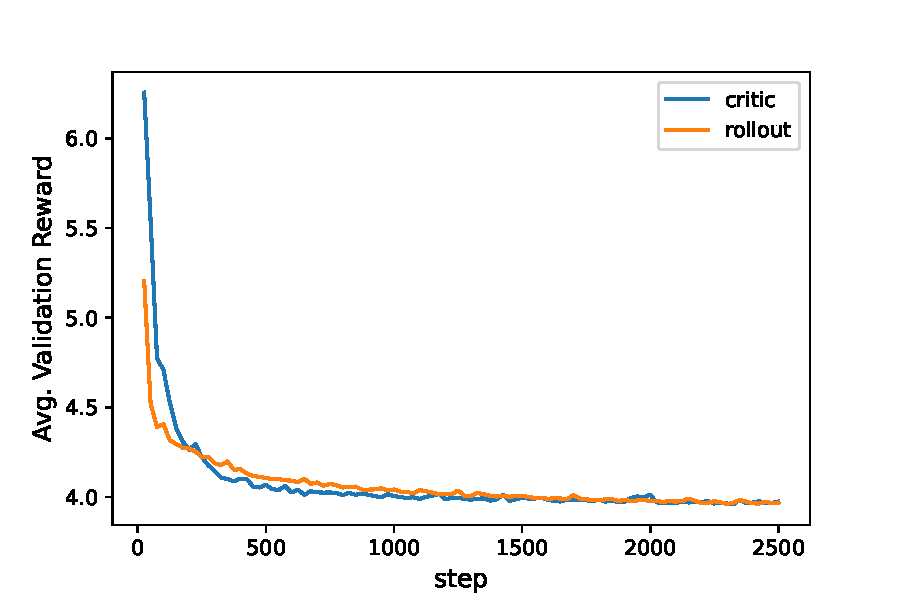
\includegraphics[width=8cm]{images/rollout-critic.pdf}
    \caption{Different baseline: greedy rollout and critic}
    \label{fig:my_label}
\end{figure}
As can be seen from the figure, the average tour length tend to lower in case of the greedy rollout baseline as compared to the learned critic baseline which validates our intuition. 
\item 
The next study involves the effect of different number of layers in the encoder part, which indicate a trade-off between
quality of the results and computational complexity (runtime) of the model and the best is achieved with $N=3$.
\begin{figure}[H]
\captionsetup[subfigure]{justification=centering}
     \centering
    \begin{subfigure}{0.48\linewidth}
         \centering
         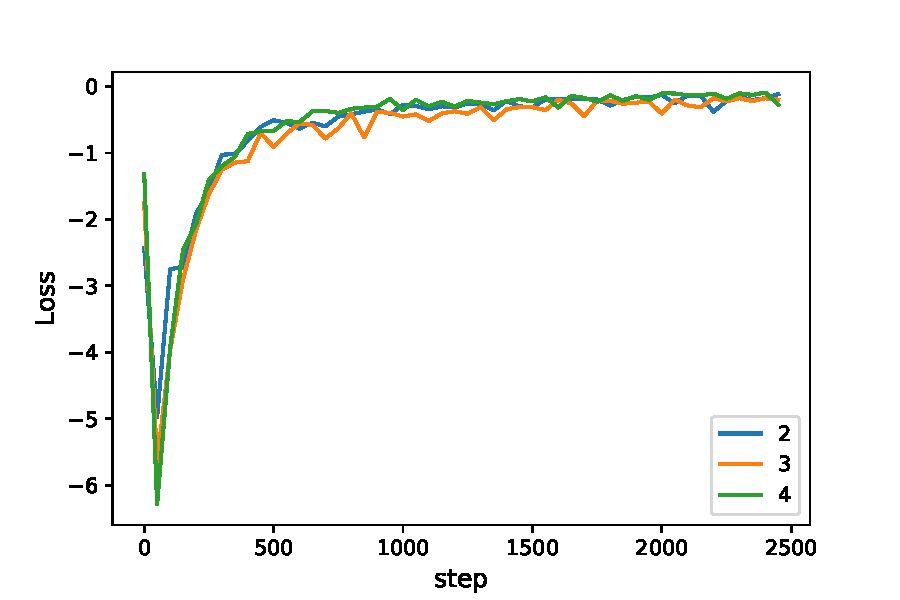
\includegraphics[width=0.9\linewidth]{images/layerloss.pdf}
         \caption{Learning Loss}
        \label{fig:bandit}
     \end{subfigure}
      \begin{subfigure}{0.48\linewidth}
         \centering
         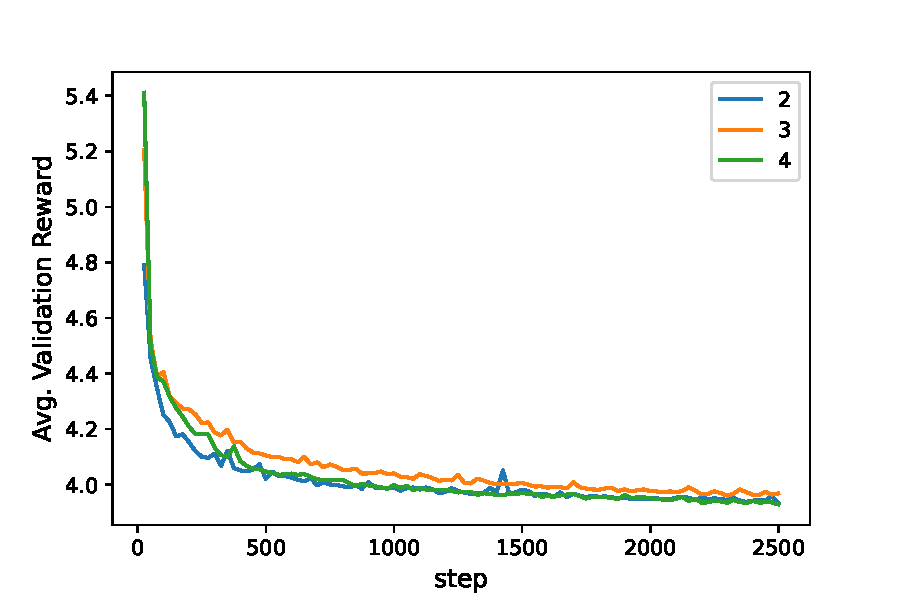
\includegraphics[width=0.9\linewidth]{images/layerreward.pdf}
         \caption{Average Reward}
        %  \label{fig:nonideal}
     \end{subfigure}
     \caption{Different Encoder Layers}
\end{figure}
\item Lastly, we validate that with higher learning rate of 0.001 the learning becomes unstable and the optimal is found to be 0.0001. \begin{figure}[H]
\captionsetup[subfigure]{justification=centering}
     \centering
    \begin{subfigure}{0.48\linewidth}
         \centering
         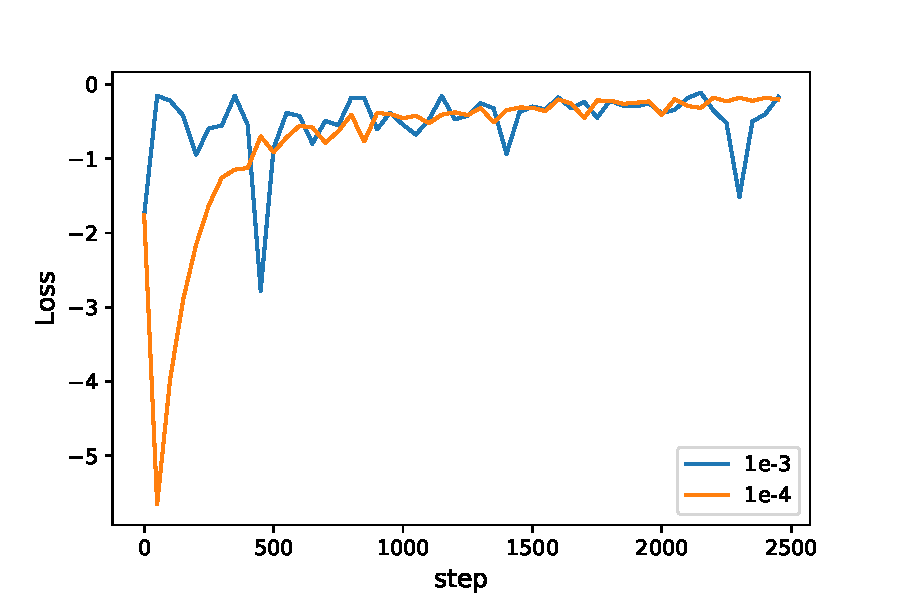
\includegraphics[width=0.9\linewidth]{images/lrloss.pdf}
         \caption{Learning Loss}
        \label{fig:bandit}
     \end{subfigure}
      \begin{subfigure}{0.48\linewidth}
         \centering
         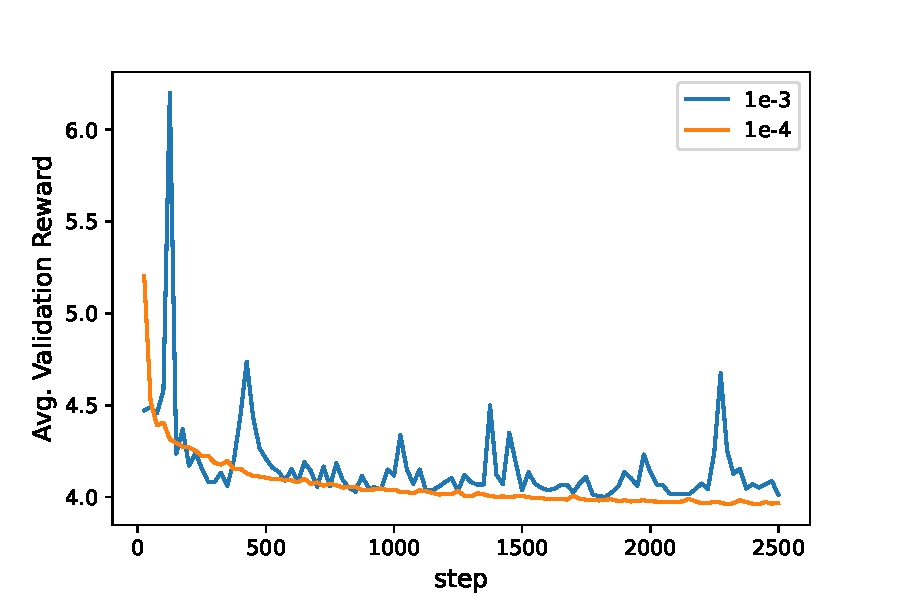
\includegraphics[width=0.9\linewidth]{images/lrreward.pdf}
         \caption{Average Reward}
        %  \label{fig:nonideal}
     \end{subfigure}
     \caption{Different Learning Rate}
\end{figure}

\end{enumerate}

Finally we show surprising results for the TSP problem with 20 and 50 nodes

\begin{figure}[H]
\captionsetup[subfigure]{justification=centering}
     \centering
    \begin{subfigure}{0.48\linewidth}
         \centering
         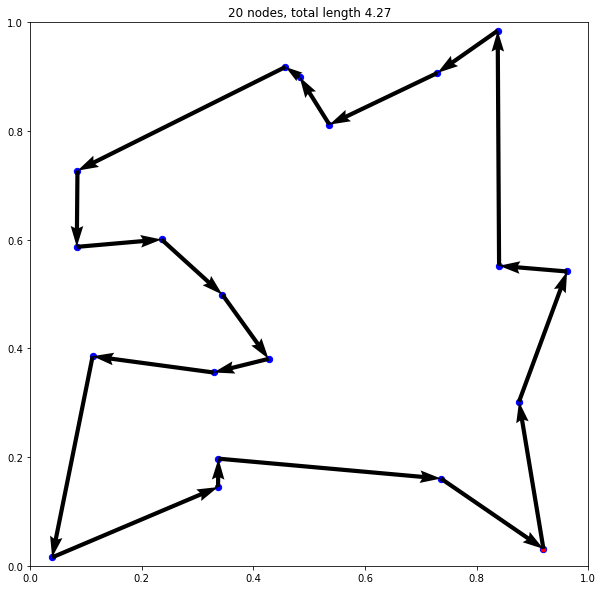
\includegraphics[width=0.65\linewidth]{images/learned_20.png}
         \caption{20 Nodes\\Tour length 4.27}
        \label{fig:bandit}
     \end{subfigure}
      \begin{subfigure}{0.48\linewidth}
         \centering
         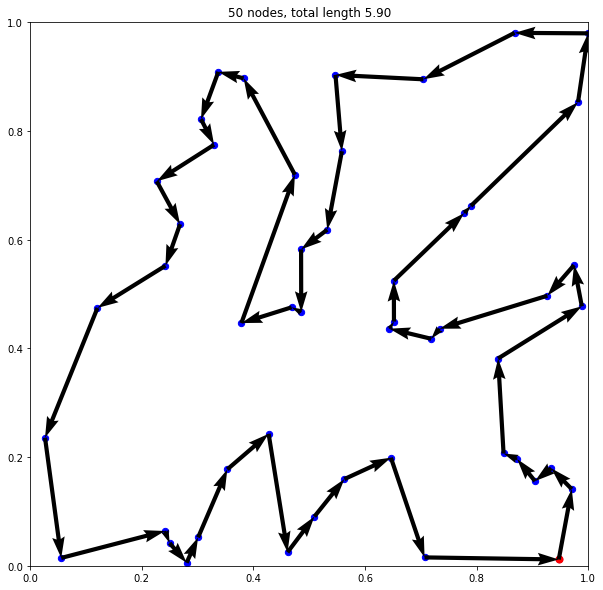
\includegraphics[width=0.65\linewidth]{images/learned_50.png}
         \caption{50 Nodes\\Tour length 5.90}
        %  \label{fig:nonideal}
     \end{subfigure}
     \caption{Solving Traveling Salesman Problem}
\end{figure}    

Our codebase for the experimentation can be found in \href{https://github.com/tejassp2002/CS769_Project}{GitHub Repository}. We have used the author's codebase for ablation study of the Attention based REINFORCE algorithm.

\bibliographystyle{unsrt}
\bibliography{references.bib}
\end{document}

